\documentclass[../main/main.tex]{subfiles}
\graphicspath{{./figures/}}

\makeatletter
\renewcommand{\@chapapp}{Travaux pratiques -- TP}
\renewcommand{\chaplett}{TP}
\makeatother

% \toggletrue{student}
% \toggletrue{corrige}
% \renewcommand{\mycol}{black}
% \renewcommand{\mycol}{gray}

\hfuzz=5.002pt

\begin{document}
\setcounter{chapter}{4}

\settype{enon}
\settype{solu_prof}
\settype{solu_stud}

\chapter{Circuits en r\'egime permanent}

\enonce{
	\begin{tcn}[sidebyside](appl)<ctb>"how"'t'{Capacités exigibles}
		\begin{itemize}[label=\rcheck]
			\item Préciser la perturbation induite par l'appareil de mesure sur le
			      montage et ses limites (bande passante, résistance d'entrée)~;
			\item Définir la nature de la mesure effectuée (valeur efficace, valeur
			      moyenne, amplitude, valeur crête à crête, etc.)~;
			\item Gérer, dans un circuit électronique, les contraintes liées à la
			      liaison entre les masses.
		\end{itemize}
		\tcblower
		\begin{itemize}[label=\rcheck]
			\item Mesurer une tension au voltmètre ou à l'oscilloscope~;
			\item Mesurer une intensité à l'ampèrementre ou à l'oscilloscope aux
			      bornes d'une résistance adaptée.~;
			\item Mesurer une résistance à l'ohmmètre ou à l'oscilloscope ou au
			      voltmètre par diviseur de tension~;
		\end{itemize}
	\end{tcn}
	\vspace{-10pt}
	\section{Objectifs}
	\begin{isd}
		\begin{itemize}
			\item Réaliser des montages électriques lisibles~;
			\item Mesurer une tension et une intensité directement à l'aide d'un
			      multimètre numérique.
		\end{itemize}
		\tcblower
		\begin{itemize}
			\item Mesurer une résistance interne de manière indirecte avec un pont
			      diviseur de tension.
			\item Réaliser une régression linéaire.
		\end{itemize}
	\end{isd}

	\begin{tcn}[cnt, bld](impo){}
		Vous prendrez soin de refaire tous les schémas des circuits mis en place ou
		étudiés.
	\end{tcn}

	\vspace{-30pt}
	\section{S'approprier}
	\subsection{Le multimètre}

	Un multimètre permet de mesurer une intensité (ampèremètre), une différence de
	potentiel (voltmètre) ou une résistance (ohmmètre). Il est nécessaire de~:
	\begin{itemize}
		\item Utiliser les bonnes bornes (la borne COM est
		      toujours utilisée).
		\item Choisir le bon mode (AC ou DC).
		\item Choisir le bon calibre.
	\end{itemize}

	\noindent
	\begin{minipage}[t]{.75\linewidth}
		~
		\begin{tcb}(defi){Les modes AC et DC}
			Le mode DC (courant continu, Direct Current), de symbole
			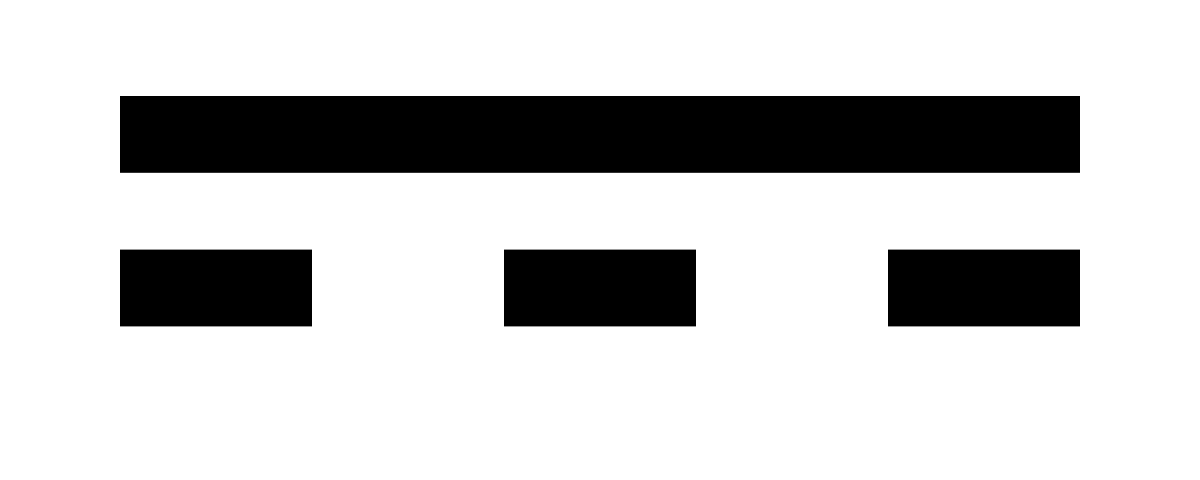
\includegraphics[height=12pt]{dc}, permet de mesurer la valeur moyenne d'une
			tension ou d'une intensité~:

			\begin{equation*}
				\left\langle s \right\rangle = \frac{1}{T} \int_{t_0}^{t_0+T} s(t) \dt
			\end{equation*}

			Le mode AC (courant alternatif, Alternating Current), de symbole
			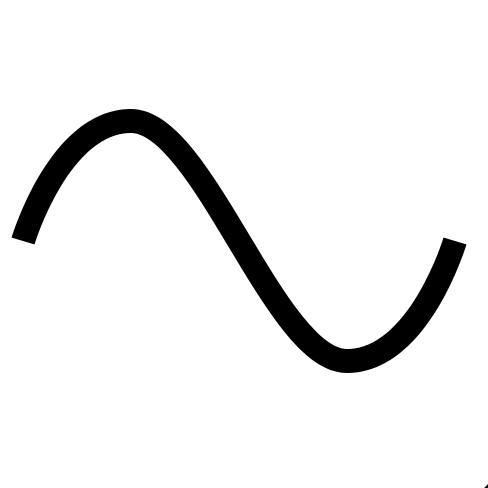
\includegraphics[height=12pt]{ac}, permet de mesurer la valeur efficace
			d'une tension ou d'une intensité~:

			\begin{equation*}
				S_{\rm eff} = \sqrt{ \left\langle s^2 \right\rangle} = \sqrt{\frac{1}{T}
					\int_{t_0}^{t_0+T} s^2(t) \dt}
			\end{equation*}
		\end{tcb}
	\end{minipage}
	\hfill
	\begin{minipage}[t]{.25\linewidth}
		\begin{center}
			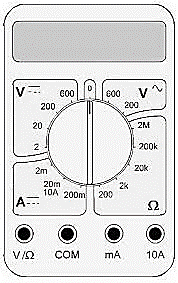
\includegraphics[width=\linewidth]{multi}
		\end{center}
	\end{minipage}

	\begin{tcb}(tool)<lftt>{Choix de calibre}
		Il faut prendre le \textbf{plus petit calibre au-dessus} de la valeur
		mesurée pour maximiser la précision de la mesure.
	\end{tcb}
	\subsection{Gestion de la masse d'un circuit}

	Dans un circuit électrique, il ne peut y avoir \textbf{qu'un seul point de
		référence des potentiels} (masse), donc il ne peut donc y avoir qu'une seule
	masse dans le circuit (sauf si on utilise un transformateur d'isolement, voir
	le prochain TP). Une bonne habitude consiste à utiliser des câbles noirs
	uniquement pour indiquer où se trouvent les masses du circuit. Tous les câbles
	noirs d'un circuit doivent alors être reliés entre eux~!

	\begin{tcb}*(impo){Couleur des fils}
		\begin{enumerate}
			\item Un fil NOIR est toujours à la masse du circuit.
			\item Un fil NOIR se branche uniquement sur un fil NOIR.
		\end{enumerate}
	\end{tcb}
}

\section{Réaliser et valider}
\enonce{%
	\subsection{Matériel}
	\begin{tcb}[sidebyside, sidebyside align=top](mate)"tool"{}
		\tcbsubtitle{\fatbox{Sur votre paillasse~:}}
		\begin{itemize}
			\item Une alimentation stabilisée.
			\item Un générateur basses fréquences.
			\item Une boîte de résistances variables\ftn{Boîte à décades.}.
			\item 2 multimètres (un Métrix et un du type de celui schématisé
			      ci-dessus, portable).
			\item Plaquette de branchement et fils.
		\end{itemize}
		\tcblower
		\tcbsubtitle{\fatbox{Sur la paillasse centrale~:}}
		\begin{itemize}
			\item Résistances de différentes valeurs~: (\SI{1}{k\ohm},
			      \SI{2.2}{k\ohm}, \SI{10}{k\ohm}, \SI{5}{M\ohm} et \SI{10}{M\ohm}).
		\end{itemize}
	\end{tcb}
}%

\setcounter{subsection}1

\subsection{Les lois de base des circuits électriques}
\subsubsection{La loi d'Ohm}

\enonce{%
	\begin{isd}[righthand ratio=.3]
		\begin{itemize}
			\item Réaliser le montage ci-contre avec une résistance $R$ de
			      \SI{10}{k\ohm}.
			\item Le générateur à utiliser est l'alimentation stabilisée variable (côté
			      tension variable). La mettre sur \SI{5}{V} environ.
			\item ATTENTION aux branchements des multimètres~!!
		\end{itemize}
		\tcblower
		\begin{center}
			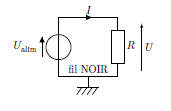
\includegraphics[width=\linewidth]{lohm}
		\end{center}
	\end{isd}
}%

\setlist[blocQR,1]{leftmargin=10pt, label=\sqenumi}
\QR{%
	Vérifier l'accord à la loi d'\textbf{Ohm} à l'aide d'une mesure de $U$
	(grâce au voltmètre «~portable~») et de $I$ (grâce au multimètre Métrix).
}{%
	solu
}%

\subsubsection{Lois des mailles et des nœuds}
\enonce{%
	\begin{isd}[righthand ratio=.3]
		\begin{itemize}
			\item Réaliser le montage ci-contre en utilisant de nouveau l'alimentation
			      stabilisée variable et en donnant aux trois résistances des valeurs
			      différentes comprises par exemple entre \SI{1}{k\ohm} et \SI{10}{k\ohm}.
		\end{itemize}
		\tcblower
		\begin{center}
			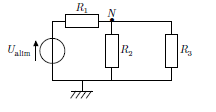
\includegraphics[width=\linewidth]{ldmn}
		\end{center}
	\end{isd}
}%

\QR{%
	Vérifier expérimentalement la loi des mailles sur la maille de gauche
	en utilisant les multimètres.
}{%
	solu
}%

\QR{%
	Vérifier aussi la loi des nœuds en N à l'aide des multimètres~(vous
	pourrez emprunter un 3\ieme{} multimètre à un-e de vos voisin-es).
}{%
	solu
}%

\subsubsection{Pont diviseur de tension}
\enonce{%
	\begin{isd}[righthand ratio=.3]
		On réalise le montage ci-contre, dans lequel $E = \SI{5}{V}$, $R_2 =
			\SI{1}{k\ohm}$ et $R_1$ est une résistance variable. Les résistances $R_1$ et
		$R_2$ étant en série, le pont diviseur de tension conduit à~: $\DS U\ind{theo} =
			\frac{R_2}{R_1+R_2}E$.
		\tcblower
		\begin{center}
			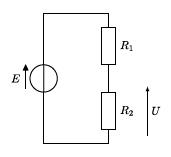
\includegraphics[width=\linewidth]{pontdiv}
		\end{center}
	\end{isd}
}%

\QR{%
	Mesurer plusieurs valeurs de la tension $U\ind{exp}$ pour plusieurs
	valeurs de la résistance $R_1$ (entre \num{0.1} et \SI{10}{k\ohm}).
}{%
	solu
}%

\QR{%
	À l'aide d'un écart \textbf{relatif}, conclure si la formule du pont
	diviseur est compatible avec les valeurs mesurées.
}{%
	solu
}%

\subsection{Résistances d'entrée et de sortie d'un dipôle}
\subsubsection{Résistance de sortie du GBF}

\enonce{%
	\begin{tcb}(impo)<lftt>{Utilisation GBF continu}
		Dans cette partie, on utilise le générateur basse fréquence (GBF) en mode
		continu (DC pour direct current) en \textbf{tirant le bouton offset} et le
		tournant de façon à lui faire délivrer \SI{5}{V} environ. Il ne faut, par
		ailleurs, qu'aucun des boutons de la ligne du haut ne soit enfoncé. On utilisera
		la sortie \SI{50}{\ohm} (aussi notée \textit{output}).
	\end{tcb}

	\begin{tcb}[sidebyside, righthand ratio=0.45](expe){R sortie GBF}
		Le GBF n'est pas une source idéale de tension~: c'est une source de tension que
		l'on peut modéliser par un générateur de Thévenin caractérisé par une
		\textit{fem} $E$ et une résistance de sortie $R_s$, comme dans la situation 1.

		Dans la situation 2, $R$ est une résistance variable (boite à décades).
		\tcblower
		\begin{center}
			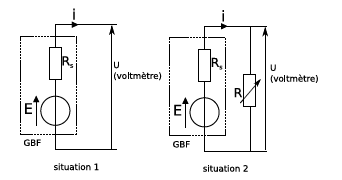
\includegraphics[width=\linewidth]{gbf}
		\end{center}
	\end{tcb}
}%

\QR{%
	Exprimer $U$ en fonction de $E$ dans la situation 1. En déduire un
	protocole de mesure de $E$.
}{%
	solu
}%

\QR{%
	Exprimer $U$ en fonction de $E$, $R$ (résistance variable) et $R_s$
	dans la situation 2. Dans le cas particulier où $U=E/2$, quelle est la
	relation entre  $R$ et $R_s$~? En déduire un protocole de mesure de
	$R_s$.
}{%
	solu
}%

\subsubsection{Résistance d'entrée d'un voltmètre}

\enonce{%
	\begin{tcb}[sidebyside, righthand ratio=.3](expe){R entrée voltmètre}
		Un voltmètre idéal est supposé de résistance infinie. Ainsi, branché
		en dérivation, il ne perturbe pas le système en absorbant une partie du
		courant. En réalité, un voltmètre possède une résistance interne grande
		mais finie, appelée résistance d'entrée du Voltmètre.

		Avec un GBF générant une tension continue, réaliser le montage
		ci-contre avec $R_1 \approx \SI{5}{M\ohm}$ et $R_2 \approx
			\SI{10}{M\ohm}$.
		\tcblower
		\begin{center}
			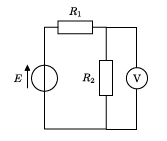
\includegraphics[width=\linewidth]{voltreel}
		\end{center}
	\end{tcb}
}%

\QR{%
	Quelle devrait être la valeur mesurée par le voltmètre, si
	celui-ci était idéal~?
}{%
	solu
}%

\QR{%
	Faire la mesure. Que pensez-vous de ce résultat~? Pouvez-vous
	donner une explication~?
}{%
	solu
}%

\QR{%
	\textbf{Conclure.}
}{%
	solu
}%

\end{document}
